\chapter{Hardware implementeringen og operativ system}\label{kap:hardware}

\begin{figure}[h]
	\vspace*{-1 cm}
	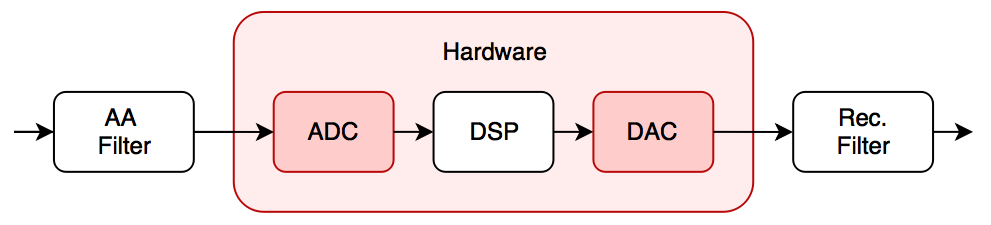
\includegraphics[width=8cm]{billeder/flow_hardware}
	\vspace{0.5 cm}
\end{figure}

\emph{I dette kapitel vil den komplette software og hardware løsning blive gennemgået som gør det muligt at udfører den digitale behandling af lydsignalet. Indledende vil de vigtigste funktioner, og dem der ligger brugeren nærmest blive gennemgået, derefter vil de enkelte lag af operativ systemet blive forklaret. Til sidst vil der være en gennemgang af de nærliggende forbedringer og optimeringer.}






